
%(BEGIN_QUESTION)
% Copyright 2011, Tony R. Kuphaldt, released under the Creative Commons Attribution License (v 1.0)
% This means you may do almost anything with this work of mine, so long as you give me proper credit

I mange mikrobølgebaserte radiosystemer brukes hule rektangulære rør, kjent som {\it bølgeledere}, ofte i stedet for kabler som overføringslinjer mellom sender/mottaker og antenne. Disse hule metallrørene fungerer som ``rør'' for å lede elektromagnetiske bølger i GHz-området med svært høy virkningsgrad, langt bedre enn koaksialkabler:

$$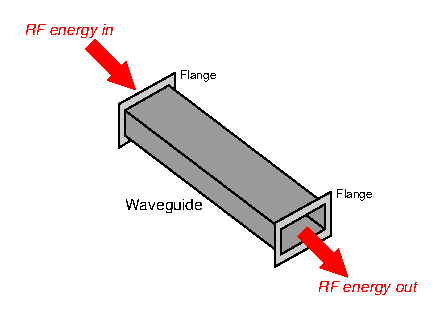
\includegraphics[width=15.5cm]{i00791x01.eps}$$

Tabellen under viser en sammenligning mellom RG-49/U bølgeleder og RG-9/U fleksibel kabel:

% No blank lines allowed between lines of an \halign structure!
% I use comments (%) instead, so that TeX doesn't choke.

$$\vbox{\offinterlineskip
\halign{\strut
\vrule \quad\hfil # \ \hfil & 
\vrule \quad\hfil # \ \hfil & 
\vrule \quad\hfil # \ \hfil \vrule \cr
\noalign{\hrule}
%
% First row
{\bf Parameter} & {\bf RG-49/U bølgeleder} & {\bf RG-9/U koaksialkabel} \cr
%
\noalign{\hrule}
%
% Another row
{\it Ytre dimensjoner} & 2 inch $\times$ 1 inch & 0.420 inch diameter \cr
%
\noalign{\hrule}
%
% Another row
{\it Dielektrikum} & luft & polyetylen (plast) \cr
%
\noalign{\hrule}
%
% Another row
{\it Vekt} & 1.4 lb per fot & 0.15 lb per fot \cr
%
\noalign{\hrule}
%
% Another row
{\it Demping ved $f$ = 5 GHz} & 0.011 dB per fot & 0.23 dB per fot \cr
%
\noalign{\hrule}
%
% Another row
{\it Effekttålighet} & 1.2 MW & 66 W \cr
%
\noalign{\hrule}
} % End of \halign 
}$$ % End of \vbox

Anta at en RG-49/U bølgeleder brukes til å overføre RF-energi fra en radartransceiver på 300 watt til en parabolantenne. Beregn RF-effekten (i watt) tilgjengelig ved antennen, forutsatt at bølgelederen er 8 fot lang og at det ikke finnes andre effekttap mellom transceiveren og antennen.

\vskip 10pt

Anta nå at radartransceiverens effekt økes til 800 watt. Beregn RF-effekten (i watt) tilgjengelig ved antennen med samme lengde på bølgelederen.

\vskip 10pt

Anta deretter at radartransceiverens effekt økes til 3 kilowatt. Beregn RF-effekten (i watt) tilgjengelig ved antennen med samme lengde på bølgelederen.

\vskip 10pt

Forblir effekttapet i bølgelederen konstant når sendeeffekten øker, eller endrer det seg med overført effekt? Hvordan viser den ``tapte'' RF-energien seg i bølgelederen (gitt at energibevaringsloven sier at energi verken kan skapes eller tilintetgjøres)?

\vskip 20pt \vbox{\hrule \hbox{\strut \vrule{} {\bf Forslag til sokratisk diskusjon} \vrule} \hrule}

\begin{itemize}
\item{} Forklar hvorfor bølgelederen over har så mye høyere effekttålighet enn koaksialkabelen, basert på deres respektive demping i dB/fot.
\item{} Hvorfor brukes ikke bølgeledere i alle radioapplikasjoner i GHz-området, når effekttapet er så mye lavere enn for koaksialkabel?
\item{} For deg som har studert nivåmåleteknologi: forklar hvordan begrepet {\it bølgeleder} henger sammen med guided-wave radar (GWR)-nivåtransmittere.
\item{} Er det mulig at en bølgeleder får {\it reflekterte signaler}, slik som en overføringslinjekabel med feil terminering? Hvorfor eller hvorfor ikke?
\end{itemize}

\underbar{file i00791}
%(END_QUESTION)





%(BEGIN_ANSWER)

$P_{antenna}$ = 293.98 W ved sendt effekt på 300 W.

\vskip 10pt

$P_{antenna}$ = 783.95 W ved sendt effekt på 800 W.

\vskip 10pt

$P_{antenna}$ = 2.9398 kW ved sendt effekt på 3 kW.

%(END_ANSWER)





%(BEGIN_NOTES)

En RG-49/U bølgeleder med lengde 8 fot vil gi en total effektdemping på:

$$(8 \hbox{ ft}) (-0.011 \hbox{ dB/ft}) = -0.088 \hbox{ dB}$$

Dette tilsvarer en demping (uttrykt som forholdstall) på:

$$10^{-0.088 \over 10} = 0.97994$$

Dermed overfører bølgelederen 97.994\% av inngangseffekten til antennen.

\vskip 10pt

Her er beregningene for effekt levert til antennen ved ulike sendereffekter:

$$(300 \hbox{ W}) (0.97994) = 293.98 \hbox{ W}$$

$$(800 \hbox{ W}) (0.97994) = 783.95 \hbox{ W}$$

$$(3000 \hbox{ W}) (0.97994) = 2939.82 \hbox{ W}$$

\vskip 10pt

Effekttapet øker med innkommende (sendt) effekt. Dette tapet viser seg vanligvis som varme, selv om noe energi også kan stråles bort fra bølgelederen (eller kabelen) som elektromagnetiske bølger, spesielt dersom det finnes åpninger i flenstetningene.

\vskip 10pt

Dataene i sammenligningen mellom bølgeleder og kabel er hentet fra {\it Electronics Manual for Radio Engineers}, første utgave, av Vin Zeluff og John Markus (1949), side 448.

















\vfil \eject

\noindent
{\bf Forberedende quiz:}

En {\it bølgeleder} er:

\begin{itemize}
\item{} Et verktøy som brukes for å justere retningsbestemte radioantenner for best mulig mottak
\vskip 5pt 
\item{} En hul metallstruktur som leder RF-energi, som en overføringslinje
\vskip 5pt 
\item{} En metallstang som gir mekanisk stivhet til en teleskopantenne
\vskip 5pt 
\item{} Et instrument laget for å måle radiosignalstyrke i én retning
\vskip 5pt 
\item{} En enhet som brukes for å roe væskeoverflaten ved nivåmåling
\vskip 5pt 
\item{} Et av elementene i en Yagi-antenne som brukes for å gjøre den mer retningsbestemt
\end{itemize}


\vfil \eject

\noindent
{\bf Forberedende quiz:}

Beregn RF-effekten tilgjengelig ved en sendeantenne (i watt) dersom senderen leverer 30 watt og kabelen mellom sender og antenne har et totalt tap på -1.3 dB.

\begin{itemize}
\item{} 1.5 watt
\vskip 5pt 
\item{} 34.2 watt
\vskip 5pt 
\item{} 22.24 watt
\vskip 5pt 
\item{} 26.33 watt
\vskip 5pt 
\item{} 28.7 watt
\vskip 5pt 
\item{} 31.3 watt
\end{itemize}


%INDEX% Electronics review: decibel power calculations
%INDEX% Electronics review: waveguides

%(END_NOTES)
